\documentclass[magick={density=600,outfile=\jobname.png}]{standalone}
\usepackage{tikz}
%\documentclass[tikz,border=5mm]{standalone}
\begin{document}
	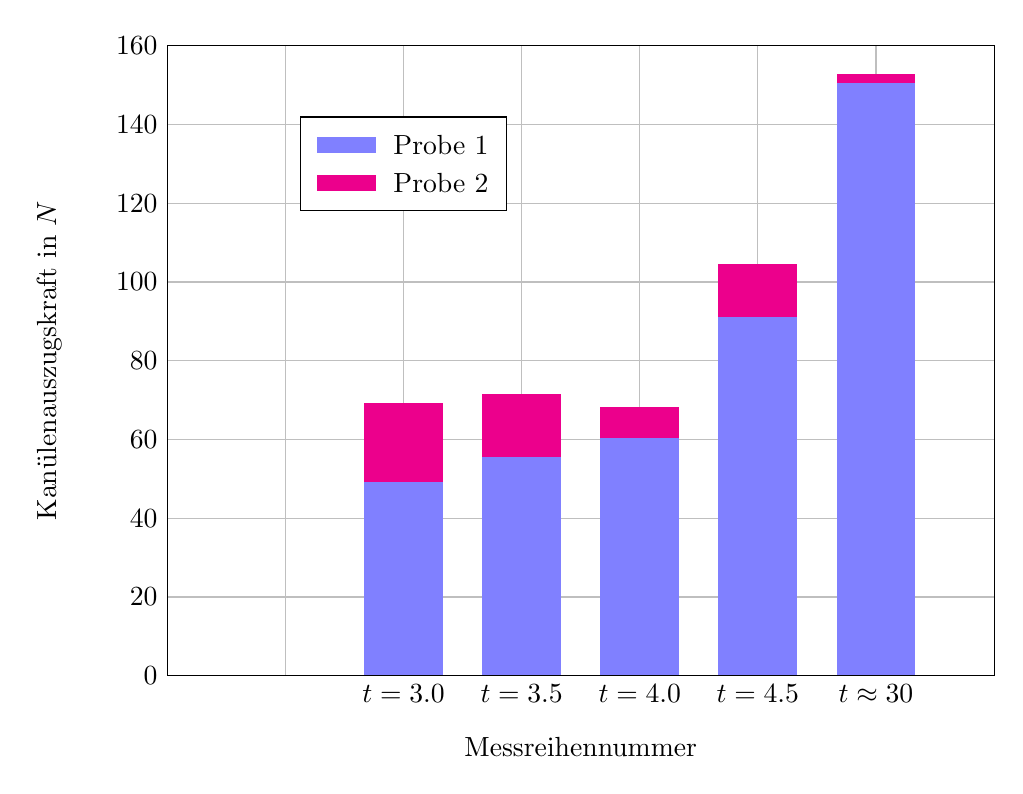
\begin{tikzpicture}[y=.5mm,x=1.5cm]
		\draw[gray!50,local bounding box=L] (0,0) grid[xstep=1.5cm,ystep=20] (7,160);
		\foreach \i/\ione/\itwo/\itext in
		{1/0/0/,
			2/49.2731776918684/19.964130020244/t=3.0,
			3/55.5745267232259/15.9911247772533/t=3.5,
			4/60.3699144999186/7.89742116804573/t=4.0,
			5/91.1499318440755/13.3824237377185/t=4.5,
			6/150.601191206667/2.13783749065102/t\approx 30
		}{
			\draw[blue!50,line width=10mm]
			(\i,0) node[below=-5mm,black]{$\itext$}--+(90:\ione) coordinate (tmp);
			\draw[magenta,line width=10mm] (tmp)--+(90:\itwo);
		}
		\foreach \i in {0,...,8}{
			\pgfmathsetmacro{\j}{int(20*\i)}
			\path (0,\j) node[left]{$\j$};
		}
		\draw (0,0) rectangle (7,160);
		\path
		(L.west)+(180:1) node[rotate=90]{Kan\"ulenauszugskraft in $N$}
		(L.south)+(-90:18) node{Messreihennummer}
		;
		% legends (as a matrix node)
		\path (2,130) node[matrix,draw,fill=white]
		{\draw[line width=2mm,blue!50] (0,0)--+(0:.5);&\node{Probe 1};\\
			\draw[line width=2mm,magenta] (0,0)--+(0:.5);&\node{Probe 2};\\};
	\end{tikzpicture}
\end{document}